\documentclass[a4paper,12pt]{article}
\usepackage[utf8]{inputenc}

%  Русский язык
\usepackage{multirow}
\usepackage{wrapfig}
\usepackage[T2A]{fontenc}			% кодировка
\usepackage[utf8]{inputenc}			% кодировка исходного текста
\usepackage[english,russian]{babel}	% локализация и переносы
\usepackage[table,xcdraw]{xcolor}
\usepackage{indentfirst} %Красная строка
\usepackage[a4paper,top=1.3cm,bottom=2cm,left=1.5cm,right=1.5cm,marginparwidth=0.5cm]{geometry}
\usepackage[usenames]{color}
\usepackage{colortbl}
\usepackage{csvsimple}
\usepackage{siunitx}
\usepackage[nottoc,notlot,notlof]{tocbibind}

\usepackage{lipsum}
\usepackage{graphicx}
 \usepackage{floatrow}

\addto\captionsrussian{\def\refname{5   Список используемой литературы}}

% Заметки
\usepackage{todonotes}

% Математика
\usepackage{amsmath,amsfonts,amssymb,amsthm,mathtools} 
\usepackage{hyperref}

\renewcommand{\AA}{\ensuremath{\mathring{A}}}

\usepackage{graphicx}
\usepackage[table,xcdraw]{xcolor}




\begin{document}
\def\figurename{Рисунок}
\begin{titlepage}
\begin{center}
    {\large МОСКОВСКИЙ ФИЗИКО-ТЕХНИЧЕСКИЙ ИНСТИТУТ (НАЦИОНАЛЬНЫЙ ИССЛЕДОВАТЕЛЬСКИЙ УНИВЕРСИТЕТ)}
\end{center}
\begin{center}
    {\largeФизтех-школа биологической и медицинской физики}
\end{center}

\vspace{1cm}
{\huge
\begin{center}
    {\bf Лабораторная работа по общей физике}\\
    \vspace{0.5cm}
    5.1.2 Эффект Комптона.
\end{center}
}

\vspace{4cm}
\begin{flushright}
{\LARGE Выполнили студенты группы Б06-103:\\ Фитэль Алена \\Флоренская Лидия\\}

\end{flushright}
\vspace{9cm}
\begin{center}
    Долгопрудный, 2023 г.
\end{center}
\end{titlepage}


\newpage
\section{Введение}



\paragraph{Цель работы:}
С помощью сцинтилляционного спектрометра исследуется энергетический спектр $\gamma$-квантов, рассеянных на графите. Определяется энергия рассеяных $\gamma$-квантов в зависимости от угла рассеяния, а также энергия покоя частиц, на которых происходит комптоновское рассеяние.\par
\begin{wrapfigure}{r}{0.3\textwidth}
	\begin{center}
		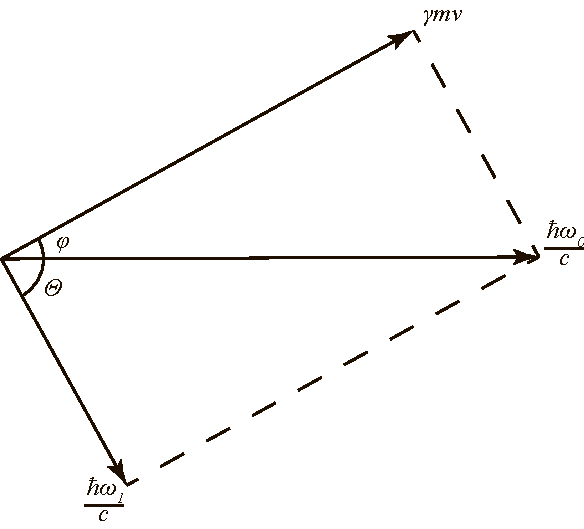
\includegraphics[width=\linewidth]{pic1.pdf}
		\caption{Векторная диаграмма рассеяния $\gamma$-кванта на электроне}
		\label{pic1}
	\end{center}
\end{wrapfigure}
Рассеяние $\gamma$-лучей в веществе относится к числу явления, в которых особенно ясно проявляется двойственная природа излучения. Волновая теория, хорошо объясняющая рассеяние длинноволонового излучения, испытывается трудности при описании рассеяния рентгеновских и $\gamma$-лучей. Эта теория, в частности, не может объяснить, почему в составе рассеянного излучения, измеренного Комптоном, кроме исходной волны с частотой $\omega_0$ появляется дополнительная длинноволновая компонента, отсутствующая в спектре первичного излучения.\par
Появление этой компоненты легко объяснимо, если считать, что $\gamma$-излучение представляет собой поток квантов (фотонов), имеющих энергию $\hbar\omega$ и импульс $p=\hbar\omega/c$. Эффект Комптона -- увеличение длинны волны рассеянного излучения по сравнению с падающим -- интерпретируется как результат упругого соударения двух частиц: $\gamma$-кванта (фотона) и свободного электрона.\par
Рассмотрим элементарную теорию эффекта Комптона. Пусть электрон до соударения (его энергия равна энергии покоя $mc^2$), а $\gamma$-квант имел начальную энергию $\hbar\omega_0$ и импульс $\hbar\omega_0/c$. После соударения электрон приобретает энергию $\gamma mc^2$ и импульс $\gamma mv$, где $\gamma=(1-\beta^2)^{-1/2},\ \beta=v/c$, а $\gamma$-квант рассеивается на некоторый угол $\theta$ по отношению к первоначальному направлению движения. Энергия и импульс $\gamma$-кванта становятся соответственно равными $\hbar\omega_1$ и $\hbar\omega_1/c$ (рис. \ref{pic1}).\par
Запишем для рассматриваемого процесса законы сохранения энергии и импульса:
\begin{equation*}
	mc^2+\hbar\omega_0=\gamma mc^2+\hbar\omega_1,
\end{equation*}
\begin{equation*}
	\frac{\hbar\omega_0}{c}=\gamma mv\cos\varphi+\frac{\hbar\omega_1}{c}\cos\theta,
\end{equation*}
\begin{equation*}
	\gamma mv\sin\varphi=\frac{\hbar\omega_1}{c}\sin\theta.
\end{equation*}
\par
Решая совместно эти уравнения и переходя от частот $\omega_0$ и $\omega_1$ к длинам волн $\lambda_0$ и $\lambda_1$, нетрудно получить, что изменение длины волны рассеянного излучения равно
\begin{equation}
	\Delta\lambda=\lambda_1-\lambda_0=\frac{h}{mc}\left(1-\cos\theta\right)=\Lambda_k\left(1-\cos\theta\right),
	\label{eq:ComptonWavelength}
\end{equation}
где $\lambda_0$ и $\lambda_1$ -- длины волн $\gamma$-кванта до и посл рассеяния, а величина
\begin{equation*}
	\Lambda_k=\frac{h}{mc}=2.42\cdot10^{-10}\text{ см}
\end{equation*}
называется комптоновской длиной волны электрона. Из формулы (\ref{eq:ComptonWavelength}) следует, что комптоновское смещение не зависит ни от длины волны первичного излучения, ни от рода вещества, в котором наблюдается рассеяние. В приведенном выводе электрон в атоме считается свободным. Для $\gamma$-квантов с энергией в несколько десятков, а тем более сотен килоэлектрон-вольт, связь электронов в атоме, действительно, мало существенна, так как энергия их связи в легких атомах не превосходит нескольких килоэлектрон-вольт, а для большинства электронов еще меньше.\par
При рассеянии на связанных электронах изменение импульса кванта воспринимается атомом в целом. Поскольку масса атома очень велика, передача импульса не сопровождается сколько-нибудь заметной передачей энергии, и наблюдается несмещенная (по энергии) компонента в спектре рассеянного излучения. Таким образом, рассеяние $\gamma$-квантов на связанных электронах можно рассматривать как упругое столкновение квантов с атомами. В классике такое рассеяние называется рэлеевским и рассматривается как процесс, при котором связанные электроны атома приходят в резонансное колебание под действием падающего излучения, а затем сами излучают фотоны той же частоты. При рассеянии квантов не очень высокой энергии ($1\div 10$ кэВ) часть электронов ведет себя, как свободные, а часть -- как связанные. Оба типа рассеяния при этом наблюдаются одновременно.\par
При увеличении атомного номера $Z$ рассеивателя сечение рэлеевского рассеяния растет как $Z^2$, тогда как сечение комптоновского рассеяния на атоме пропорционально $Z$. Это происходит по следующей причине. При комптоновском рассеянии каждый электрон атома ведет себя независимо от других, поскольку рассеяние в этом случае происходит на каком-либо одном из атомных электронов. При рэлеевском рассеянии фотоны излучаются всеми (или почти всеми) электронами атомной оболочки, колеблющимися синфазно. Их излучение когерентно, так что складываются амплитуды, а не интенсивности излученных волн электронов.\par

\begin{wrapfigure}{l}{0.4\textwidth}
	\begin{center}
		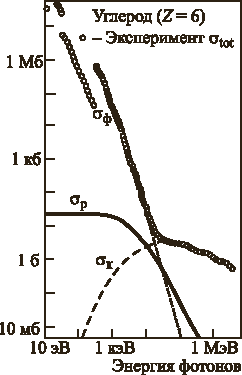
\includegraphics[scale=1.2]{pic2.pdf}
		\caption{Сечение взаимодействия фотонов с углеродом ($Z=6$) при энергиях фотона от 10 эВ до 1 МэВ; $\sigma_{\text{ф}}$ -- сечение фотоэффектра, $\sigma_{\text{р}}$ -- сечение рэлеевского рассеяния, $\sigma_{\text{к}}$ -- сечение комптоновского рассеяния; $\sigma_{\text{tot}}$ -- полное сечение взаимодействия фотнов с ядром углерода}
		\label{pic2}
	\end{center}	
\end{wrapfigure}
Сечение комптоновского и рэлеевского рассеяний по-разному зависят и от энергии фотонов. С увеличением энергии сечение рэлеевского рассеяния уменьшается очень быстро, а сечение комптоновского рассеяния -- незначительно.\par
Это различие в энергетической зависимости комптоновского $\sigma_{\text{к}}$ и рэлеевского $\sigma_{\text{р}}$ сечений рассеяний показано на рис. \ref{pic2}. Обратите внимание на то, что при рассеянии на углероде рентгеновских квантов с энергией $\simeq 20$ кэВ (как это было в эксперименте Комптона) $\sigma_{\text{к}}$ порядка $\sigma_{\text{р}}$, и поэтому наблюдаются две линии -- смещенная и несмещенная. В то же время при рассеянии на углероде фотонов с энергией $\simeq 600$ кэВ (которые используются в данной работе) $\sigma_{\text{к}} \gg \sigma_{\text{р}}$, и поэтому наблюдается только смещенная компонента. Сечение рэлеевского рассеяния на атоме, при уменьшении длины волны уменьшается пропорционально $\lambda^2$ вследствие интерференции излучения, рассеянного от различных участков распределения.



\par

В заключение укажем, что кроме рассеяния $\gamma$-кванты испытывают в среде поглощение, вызываемое фотоэффектом и рождение электрон-позитронных пар. Процесс рождения пар пороговых, он возможен лишь при энергии $\gamma$-квантов больше $2mc^2=1.02$ МэВ и в рассматриваемом энергетическом диапазоне не происходит. При фотоэффекте из атома выбивается электрон, а квант поглощается. Импульс кванта делится между вылетевшим электроном и атомом, а его энергия частично передается электрону, а частично тратится на возбуждение атома. Атом практически мгновенно (за время порядка $10^{-8}$ с) возвращается в нормальное состояние. Его энергия возбуждения либо излучается в виде мягкого фотона, либо передается какому-нибудь другому электрону, который покидает атом (Оже-эффект). И в том, и в другом случае энергия возбуждения обычно поглощается соседними атомами рассеивателя.\par



Основной целью данной работы является проверка соотношения (\ref{eq:ComptonWavelength}). Применительно к условиям нашего опыта формулу (\ref{eq:ComptonWavelength}) следует преобразовать от длин волн к энергии $\gamma$-квантов. Как нетрудно показать, соответствующее выражение имеет вид
\begin{equation}
	\frac{1}{\varepsilon(\theta)}-\frac{1}{\varepsilon_0}=1-\cos\theta.
	\label{eq2}
\end{equation}
\par
Здесь $\varepsilon_0=E_0/\left(mc^2\right)$ -- выраженная в единицах $mc^2$ энергия $\gamma$-квантов, падающих на рассеиватель, $\varepsilon(\theta)$ -- выраженная в тех же единицах энергии квантов, испытавших комптоновское рассеяние на угол $\theta$, $m$ -- масса электрона.
\section{Экспериментальная установка}
Блок-схема установки изображена на рис. \ref{scheme}. Источником излучения 1 служит $^{137}$Cs, испускающий $\gamma$-лучи с энергией 662 кэВ. Он помещен в толстостенный свинцовый контейнер с коллиматором. Сформированный коллиматором узкий пучок $\gamma$-квантов попадает на графитовую мишень 2 (цилиндр диаметром 40 мм и высотой 100 мм).
\begin{figure}[!htb]
	\centering
	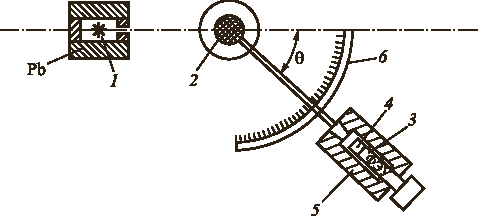
\includegraphics[scale=1.2]{scheme.pdf}
	\caption{Блок-схема установки по изучению рассеяния $\gamma$-квантов}
	\label{scheme}
\end{figure}
\par
Кванты, испытавшие комптоновское рассеяние в мишени, регистрируются сцинтилляционным счетчиком. Счетчик состоит из фотоэлектронного умножителя 3 (далее ФЭУ) и сцинтиллятора 4. Сцинтиллятором служит кристалл NaI(Tl) цилиндрической формы диаметром 40 мм и высотой 40 мм, его выходное окно находится в оптическом контакте с фотокатодом ФЭУ. Сигналы, возникающие на аноде ФЭУ, подаются на ЭВМ для амлитудного анализа. Кристалл и ФЭУ расположены в светонепроницаемом блоке, укрепленном на горизонтальной штанге. Штанга вместе с этим блоком может вращаться относительно мишени, угол поворота отситывается по лимбу 6.\par
Головная часть сцинтилляционного блока закрыта свинцовым коллиматором 5, который формирует входной пучок и защищает детектор от постороннего излучения. Основной вклад в это излучение вносят $\gamma$-кванты, проходящие из источника 1 через 6-сантиметровые стенки защитного контейнера. Этот фон особенно заметен при исследовании комптоновского рассеяния на большие углы ($\simeq 120^\circ$), когда расстояние между детектором и источником уменьшается.
\section{Ход работы}

\begin{enumerate}
	\item Включим все измерительные устройства и компьютер.
	\item Запустим программу и войдем в режим измерения спектра.
 \newpage
	\item Проверим функционировании установки в этом режиме при малом времени экспозиции (порядка 1 минуты):
	\begin{enumerate}
		\item снимем спектр при $\theta=0^\circ$;
		\item установим угол $\theta\simeq 30^\circ$ и снова снимем спектр, убедимся в том, что фотопик смещается влево, в сторону меньших энергий;
		\item определим положения фотопиков (номера канала) на экране дисплея.
	\end{enumerate}
	\item Устанавливая сцинтилляционный счетчик под разными углами $\theta$ к первоначальному направлению полета $\gamma$-квантов и вводя значения этих углов в ЭВМ, снимем амплитудные спектры и определим положение фотопиков для каждого значения угла $\theta$, аппроксимировав полученные функции распределения гауссовскими кривыми (Рисунок ). Погрешность определения этих положений примем равной среднеквадратичной погрешности отклонения от полученного расперделения, соответсявующего даннному набору данных. Измерения проводим с шагом $10^\circ$ в диапазоне от $0^\circ$ до $120^\circ$. Результаты измерений и экстарполяций занесем в Таблицу \ref{tab:my-table}.

\begin{figure}[!h]
		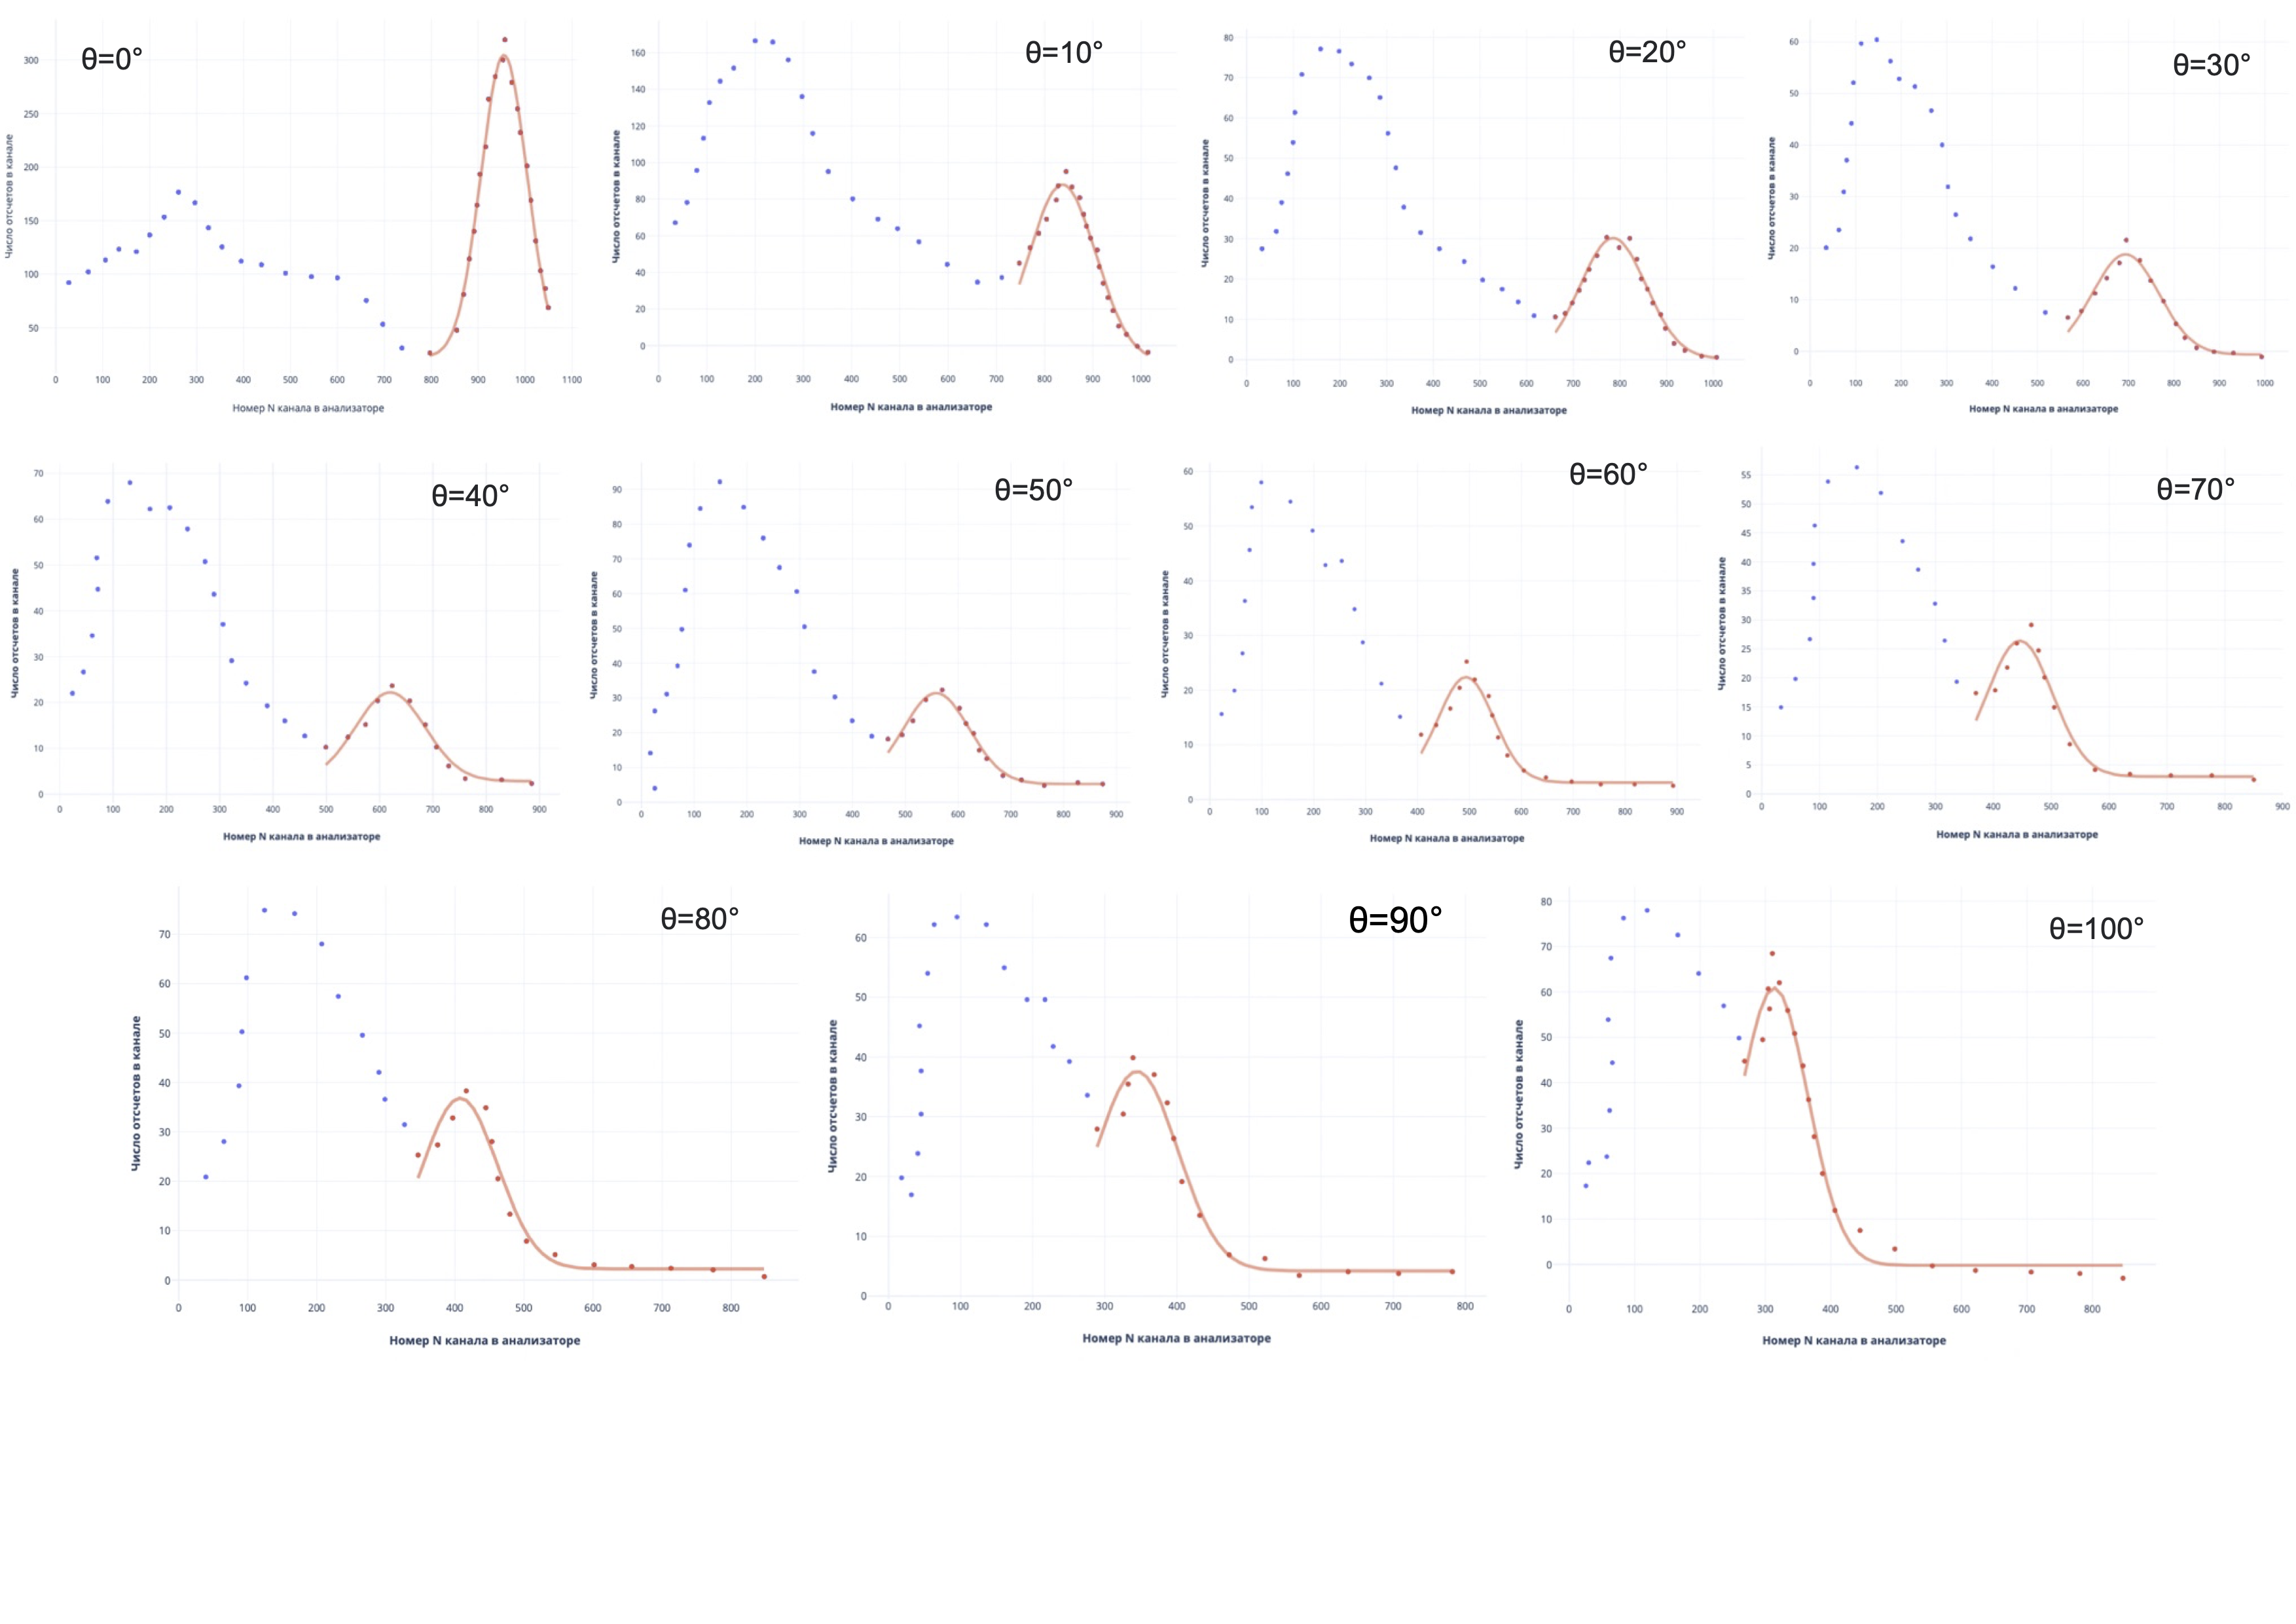
\includegraphics[width=\textwidth]{4.png}
		\caption{Аппроксимация гистограмм числа импульсов от значений их модулей гауссовскими кривыми. }
		\label{fig:graph}
	\end{figure}
 
		



\begin{table}[h!]
\centering
\begin{tabular}{|r|r|r|r|r|}
\hline
\textbf{$N$} & \textbf{$\sigma N$} & \textbf{$\theta, $} град. & \textbf{$1 - \cos(\theta)$} & \textbf{$\sigma (1 - \cos(\theta))$} \\ \hline
960 & 50 & 0   & 0.000     & 0.000     \\ \hline
840 & 70 & 10  & 0.015 & 0.003 \\ \hline
790 & 70 & 20  & 0.060  & 0.006 \\ \hline
690 & 70 & 30  & 0.134 & 0.009 \\ \hline
620 & 70 & 40  & 0.234 & 0.011 \\ \hline
560 & 40 & 50  & 0.357 & 0.013 \\ \hline
490 & 50 & 60  & 0.500   & 0.015 \\ \hline
450 & 60 & 70  & 0.658 & 0.016 \\ \hline
410 & 50 & 80  & 0.826 & 0.017 \\ \hline
340 & 60 & 90  & 1.000     & 0.017 \\ \hline
310 & 50 & 100 & 1.174 & 0.017 \\ \hline
\end{tabular}
\caption{Распределение номеров каналов $N$, соответствующих фотопикам для разных углов рассеяния $\theta$}
\label{tab:my-table}
\end{table}





 
	\item Используя экспериментальные результаты, построим график (рис. \ref{fig:graph}), откладывая по оси абсцисс величину $1-\cos\theta$, а по оси ординат величину $1/N(\theta)$. Проведем через полученные точки прямую методом взвешенного МНК.


	\begin{figure}[!htb]
		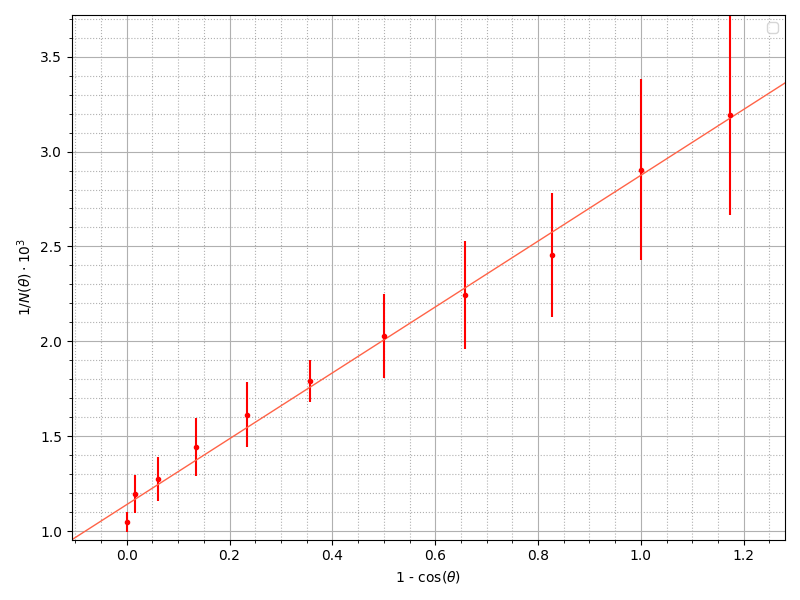
\includegraphics[width=\textwidth]{5.1.2(2).png}
		\caption{График зависимости $\frac{1}{N}=f\left(1-\cos\theta\right)$}
		\label{fig:graph}
	\end{figure}
 \newpage
	\item Заменим в формуле \ref{eq2} энергию квантов, испытавших комптоновское рассеяние на угол $\theta$, номером канала $N(\theta)$, соответствующего вершине фотопика при указанном угле $\theta$. Обозначая буквой $A$ неизвестный коэффициент пропорциональности между $\varepsilon(\theta)$ и $N(\theta)$, найдем:
	\begin{equation}
		\frac{1}{N(\theta)}-\frac{1}{N(0)}=A(1-\cos\theta).
		\label{eq:3}
	\end{equation}
	\par
	Согласно формуле (\ref{eq:3}) экспериментальные точки должны лежать на одной прямой. Пересечение этой прямой с осью ординат определяет наилучшее значение $N_{\text{наил}}(0)$. Это значение учитывает не только непосредственно измеренную величину $N(0)$, но и измерения сделанные под другими углами, а пересечение линии с прямой $\cos\theta=0$ позволяет найти наилучшее значение $N_{\text{наил}}(90)$. Таким образом можно найти энергию покоя частиц, на которых происходит комптоновское рассеяние. Снова обратимся к формуле (\ref{eq2}). Возвращаясь от переменной $\varepsilon$ к энергии $E$, мы получаем, что при $\theta=90^\circ$ формула (\ref{eq2}) принимает вид
	\begin{equation*}
		mc^2\left(\frac{1}{E(90)}-\frac{1}{E(0)}\right)=1,
	\end{equation*}
	или
	\begin{equation}
		mc^2=E(0)\frac{E(90)}{E(0)-E(90)}=E_\gamma\frac{N(90)}{N(0)-N(90)}.
		\label{eq:4}
	\end{equation}
	где $E(0)=E_\gamma$ -- энергия электронов, рассеянных вперед -- равна энергии $\gamma$-лучей, испускаемых источником ($^{137}$Cs).\par
	\item С помощью графика \ref{fig:graph} и формулы \ref{eq:4} определим энергию покоя частицы, на которой происходит комптоновское рассеяние первичных $\gamma$-квантов:
Уравнение графика \ref{fig:graph}:
\[\frac{1}{N}=\frac{1}{N(0)} + A(1-\cos\theta),    \frac{1}{N(0)} = (1.14 \pm 0.05) \cdot 10^{-3},     A = (1.73 \pm 0.05) \cdot 10^{-3} \]

Номера каналов $N_{\text{наил}}(0), N_{\text{наил}}(90)$:

\[\begin{array}{l}
N_{\text{наил}}(0) = \dfrac{1}{\frac{1}{N(0)}} = 1140 \pm 40,\\[12pt]
N_{\text{наил}}(90) = \dfrac{1}{\frac{1}{N(0)}+A} = 348 \pm 12,\\
\end{array}
\]


Энергия покоя и масса частиц, на которых происходит Комптоновское рассеяние:
\[
mc^2=E_\gamma\frac{N(90)}{N(0)-N(90)} =E_\gamma\frac{N_{\text{наил}}(90)}{N_{\text{наил}}(0)-N_{\text{наил}}(90)} = 662 \cdot \frac{348}{792} = 291 \pm 15 \text{ кЭв},
\]
\[m = \frac{mc^2}{c^2} = (5.2 \pm 0.3)\cdot 10^{-31} \text{ кг} .\]

\end{enumerate}
\section{Обсуждение результатов и выводы}
\begin{itemize}
    \item В ходе работы наблюдалось рассеяние гамма-квантов на электронах графита. Был установлен вид диаграммы направленности излучения источника$\gamma$-квантов:при больших углах обнаруживаются фоновые $\gamma$-кванты, проходящие через боковую стенку источника.
    \item Было проведено измерение амплитудных спектров вылетающих вследствие эффекта Компнона электронов, и определено положение фотопиков для каждого значения угла $\theta$, методом аппроксимации данных гауссовскими кривыми. По полученным значениям пиков была построена их зависимость  от угла, в точности до нормировочного множителя совпадающая с зависимостью длины волны рассейнных гамма-квантов по прошествию эффекта Комптона от угла рассейяния.
    \item  Проведена оценка массы покоя частиц, на которых происходит Комптоновское рассеяние в нашей установке: $m =  (5.2 \pm 0.3)\cdot 10^{-31} \text{ кг}$.
    

    
\end{itemize}


\end{document}

\end{document}















\end{document}
